% Logics & Symbolic AI (CSC_5AI01_TP) -- one A4 sheet, recto-verso cheat sheet
% Notation follows the course slides. Build: pdflatex logic-cheatsheet.tex (twice)
\documentclass[10pt]{article}
\usepackage[a4paper,landscape,margin=0.3cm]{geometry}
\usepackage[T1]{fontenc}
\usepackage{mathptmx}
\usepackage{amsmath,amssymb}
\usepackage{multicol}
\usepackage{xcolor}
\usepackage{tikz}
\usepackage{enumitem}
\usepackage{array}
\makeatletter
\newcommand{\needspace}[1]{\par\penalty-100\begingroup\setlength{\dimen@}{#1}\vskip\z@\@plus\dimen@\penalty-100\vskip\z@\@plus-\dimen@\vskip\dimen@\penalty9999\vskip-\dimen@\vskip\z@skip\endgroup}
\makeatother
\pagestyle{empty}
\setlength{\parindent}{0pt}
\setlength{\parskip}{0pt}
\setlength{\columnsep}{6pt}
\setlength{\columnseprule}{0.3pt}
\setlength{\tabcolsep}{1.6pt}
\renewcommand{\arraystretch}{0.95}
\setlength{\abovedisplayskip}{1pt}\setlength{\belowdisplayskip}{1pt}
\definecolor{h1}{HTML}{1F4E79}\definecolor{h2}{HTML}{A23B2A}\definecolor{bg}{HTML}{EAF0F6}
\setlist{nosep,leftmargin=6.5pt,labelsep=2pt,itemsep=0pt,topsep=0pt,partopsep=0pt,parsep=0pt}
\setlist[itemize]{label={\color{h2}\scriptsize$\bullet$}}
\setlist[itemize,2]{label={\color{h2}--},leftmargin=7pt}
\newcommand{\sect}[1]{\par\vspace{1.5pt}\noindent\colorbox{h1}{\parbox{\dimexpr\linewidth-2\fboxsep}{\bfseries\color{white}#1}}\par\vspace{0.8pt}}
\newcommand{\sub}[1]{\needspace{2.2\baselineskip}\vspace{0.8pt}{\bfseries\color{h2}#1}\par\nopagebreak}
\newcommand{\kw}[1]{\textbf{#1}}
\newcommand{\cnt}[1]{{\color{h2}\bfseries(#1)}}
\newcommand{\n}[1]{\,{\color{h2}\bfseries#1)}\,}
\newcommand{\ex}[1]{\par\vspace{0.8pt}\noindent\colorbox{bg}{\parbox{\dimexpr\linewidth-2\fboxsep}{#1}}\par\vspace{0.5pt}}
\newcommand{\impl}{\supset}
\newcommand{\up}{^{\uparrow}}
\newcommand{\dn}{^{\downarrow}}
\newcommand{\gd}[1]{[#1]}
\newcommand{\gc}[1]{\langle #1\rangle}
\newcommand{\infr}[2]{\dfrac{#1}{#2}}
\begin{document}
\fontsize{8}{8.9}\selectfont
\begin{multicols*}{4}
\raggedcolumns
\raggedright
{\centering\fontsize{9}{10}\selectfont\bfseries\color{h1} Logics \& Symbolic AI -- cheat sheet\par}

%=====================================================================
\sect{1 Propositional logic}
\begin{itemize}
\item \kw{Syntax} = manipulating symbols; \kw{semantics} = meaning.
\item Formula: symbol $p$, constants $T,\bot$; $(\neg F)$; $(A\bullet B)$.
\item Syntactic/semantic: $\neg$/Not, $\wedge$/And, $\vee$/Or, $\impl$/$\Rightarrow$, $\subset$/$\Leftarrow$, $\equiv$/$\Leftrightarrow$, $\uparrow$/Nand, $\downarrow$/Nor.
\item \kw{Valuation} $v:F\to\{True,False\}$, consistent \cnt{4}: \n1$v(T)=True$ \n2$v(\bot)=False$ \n3$v(\neg F)=$ Not $v(F)$ \n4$v((A\bullet B))=v(A)\blacksquare v(B)$.
\item \kw{Tautology}: $v(X)=True$ for every $v$.
\item \kw{Satisfiable} $S$: some $v_0$ makes all $X\in S$ True (SAT).
\item $X$ tautology $\iff\neg X$ not satisfiable.
\item \kw{Consequence} $S\models X$: every $v$ satisfying $S$ makes $X$ True.
\item \kw{Key}: $S\models X\iff S\cup\{\neg X\}$ not satisfiable.
\item Ex falso: $A,\neg A\in S\Rightarrow S\models X$ for all $X$.
\item Monotony: $S\models X\Rightarrow S\cup\{A\}\models X$.
\item Deduction: $S\cup\{X\}\models Y\iff S\models(X\impl Y)$.
\item $X$ taut.\ $\iff T\impl X$ taut., since $v(T\impl X)=v(X)$.
\end{itemize}

\sect{2 CNF \& resolution}
\begin{itemize}
\item \kw{Negation normal form}: $\neg$ only before symbols.
\item $\gd{X_1..X_n}$ = generalized disjunction ($v(\gd{})=False$).
\item $\gc{X_1..X_n}$ = generalized conjunction ($v(\gc{})=True$).
\item \kw{CNF} $\gc{C_1,..,C_n}$, each \kw{clause} $C_i=\gd{\ldots}$.
\end{itemize}
\begin{tabular}{@{}l@{\ \ }l@{\ \ }l@{}}
 & rewrite & negation\\\hline
$\wedge$ & $X\wedge Y$ & $\neg X\vee\neg Y$\\
$\vee$ & $X\vee Y$ & $\neg X\wedge\neg Y$\\
$\impl$ & $\neg X\vee Y$ & $X\wedge\neg Y$\\
$\subset$ & $X\vee\neg Y$ & $\neg X\wedge Y$\\
$\uparrow$ & $\neg X\vee\neg Y$ & $X\wedge Y$\\
$\downarrow$ & $\neg X\wedge\neg Y$ & $X\vee Y$\\
$\not\supset$ & $X\wedge\neg Y$ & $\neg X\vee Y$\\
$\not\subset$ & $\neg X\wedge Y$ & $X\vee\neg Y$\\
\end{tabular}
\begin{itemize}
\item Disjunction: $\gd{..P..}\to\gd{..A,B..}$.
\item Conjunction: $\gd{..P..}\to\gd{..A..},\gd{..B..}$.
\item $\neg\neg P\to P$, $\neg T\to\bot$, $\neg\bot\to T$.
\item \kw{Resolution}: $\gd{A,X,B}$ + $\gd{C,\neg X,D}$ $\to\gd{A,B,C,D}$.
\item Proof of $X$: start $\gd{\neg X}$, end with $\gd{}$.
\item For $S\vdash X$: start $\gd{S_1},..,\gd{S_n},\gd{\neg X}$.
\item $X$ tautology $\iff$ $X$ has a resolution proof.
\item Prolog \texttt{A :- B} $=\gd{A,\neg B}$.
\end{itemize}
\ex{\textbf{Ex.} $((A\impl B)\impl(A\impl C))$\\
$\gc{\gd{\neg(A\impl B),A\impl C}}\to\gc{\gd{A\wedge\neg B,A\impl C}}$\\
$\to\gc{\gd{A,\neg A,C},\gd{\neg B,\neg A,C}}\to\gc{\gd{\neg B,\neg A,C}}$}
\begin{itemize}
\item \kw{Backward} chaining: from goal (resolution).
\item \kw{Forward} chaining: from assumptions (Hilbert, modus ponens $\frac{X\ \ X\impl Y}{Y}$).
\item $\models$ semantic (truth tables); $\vdash$ syntactic (proofs).
\item \kw{Sound}: $S\vdash F\Rightarrow S\models F$.
\item \kw{Complete}: $S\models F\Rightarrow S\vdash F$.
\end{itemize}

%=====================================================================
\sect{3 First-order logic}
\begin{itemize}
\item \kw{Terms}: variables, constants, functors $f(t_1..t_n)$.
\item \kw{Atomic formula}: predicate $p(t_1..t_n)$, arity $n$.
\item Formulas: atomic, $\neg F$, $(F\circ G)$, $(\forall x)F$, $(\exists x)F$.
\item \kw{Functor or predicate?} Inside an argument $\Rightarrow$ functor. At formula level ($\neg,\wedge,\impl$, quantifier) $\Rightarrow$ predicate.
\item \kw{Free} $v$ \cnt{4 rules}: \n1occurs in atomic $F$ \n2in $(\diamond v')F$ iff free in $F$ and $v\neq v'$ \n3in $\neg F$ iff in $F$ \n4in $F_1\circ F_2$ iff in $F_1$ or $F_2$.
\item \kw{Closed} formula: no free variable.
\end{itemize}
\sub{Semantics}
\begin{itemize}
\item Domain $D\neq\emptyset$; interpretation $I$ \cnt{3}: \n1$c^I\in D$ \n2$f^I:D^n\to D$ \n3$p^I$ $n$-ary relation.
\item Assignment $A$: $v^A\in D$. Model $M(D,I)$.
\item \kw{Attitude}: $p(t_1..)^{I,A}=True$ iff $(t_1^{I,A},..)\in p^I$.
\item $(\forall x)F$: True for all $B$ equal to $A$ save for $x$; $\exists$: for one.
\item \kw{Valid}: true in every model (all $A$).
\item $F$ valid $\iff\{\neg F\}$ not satisfiable.
\item Valid: $((\forall x)p(a,x))\impl p(a,a)$.
\item Not valid: $(\forall x)(p(a,x)\impl p(a,a))$, $(\forall x)(\exists y)p(x,y)$.
\end{itemize}
\sub{Prenex (rename variables first)}
\begin{itemize}
\item $\neg(\exists v)A\equiv(\forall v)\neg A$;\quad $\neg(\forall v)A\equiv(\exists v)\neg A$.
\item $((Qv)A\wedge B)\equiv(Qv)(A\wedge B)$, either side, $Q\in\{\forall,\exists\}$.
\item $((\forall v)A\impl B)\equiv(\exists v)(A\impl B)$ \ (flips!).
\item $((\exists v)A\impl B)\equiv(\forall v)(A\impl B)$ \ (flips!).
\item $(A\impl(Qv)B)\equiv(Qv)(A\impl B)$ \ (kept).
\end{itemize}
\sub{Skolemization}
\begin{itemize}
\item $..(\exists x_k)..F\to F(x_k/f(x_1..x_{k-1}))$, new functor.
\item Arity = number of $\forall$ before it (0 = constant).
\item Preserves satisfiability; put $\exists$ first if you can.
\item $(\forall x)(m(x)\impl(\exists y)s(x,y))\to(\forall x)(m(x)\impl s(x,f(x)))$.
\end{itemize}
\sub{Prove $F$ valid by resolution \cnt{6 steps}}
\begin{enumerate}[leftmargin=8pt]
\item $\neg F$ in prenex form (rename variables).
\item Skolemize; \n3drop $\forall$; \n4CNF (optional).
\setcounter{enumi}{4}
\item Resolution + \kw{unification} ($P(x),\neg P(c)$: $x=c$).
\item $\gd{}$ $\Rightarrow\{\neg F\}$ unsat $\Rightarrow F$ valid.
\end{enumerate}
\begin{itemize}
\item Prop.: sound, complete, \kw{decidable}.
\item FOL: sound, complete, \kw{semi-decidable} (valid $\Rightarrow$ proof found in finite time; not valid $\Rightarrow$ may never stop).
\end{itemize}

\sect{4 Natural deduction}
\renewcommand{\arraystretch}{2.15}
\begin{tabular}{@{}l@{\,}c@{\ \ }l@{\,}c@{}}
Ax & $\infr{}{\Gamma,p\vdash p}$ & $\neg$I & $\infr{\Gamma,p\vdash\bot}{\Gamma\vdash\neg p}$\\
$\neg$E & $\infr{\Gamma\vdash p\quad\Gamma\vdash\neg p}{\Gamma\vdash\bot}$ & Abs & $\infr{\Gamma,\neg p\vdash\bot}{\Gamma\vdash p}$\\
$\bot$E & $\infr{\Gamma\vdash\bot}{\Gamma\vdash p}$ & $\to$I & $\infr{\Gamma,p\vdash q}{\Gamma\vdash p\to q}$\\
$\to$E & $\infr{\Gamma\vdash p\to q\quad\Gamma\vdash p}{\Gamma\vdash q}$ & $\wedge$I & $\infr{\Gamma\vdash p\quad\Gamma\vdash q}{\Gamma\vdash p\wedge q}$\\
$\wedge$Eg & $\infr{\Gamma\vdash p\wedge q}{\Gamma\vdash p}$ & $\wedge$Ed & $\infr{\Gamma\vdash p\wedge q}{\Gamma\vdash q}$\\
$\vee$Ig & $\infr{\Gamma\vdash p}{\Gamma\vdash p\vee q}$ & $\vee$Id & $\infr{\Gamma\vdash q}{\Gamma\vdash p\vee q}$\\
\multicolumn{4}{@{}l@{}}{$\vee$E\ \ $\infr{\Gamma\vdash p\vee q\quad\Gamma,p\vdash r\quad\Gamma,q\vdash r}{\Gamma\vdash r}$}\\
$\forall$I & $\infr{\Gamma\vdash F}{\Gamma\vdash\forall xF}$ & $\forall$E & $\infr{\Gamma\vdash\forall xF(x)}{\Gamma\vdash F[t/x]}$\\
$\exists$I & $\infr{\Gamma\vdash F(t)}{\Gamma\vdash\exists xF(x)}$ & $\exists$E & $\infr{\Gamma\vdash\exists xF\quad\Gamma\vdash F\to G}{\Gamma\vdash G}$\\
\end{tabular}
\renewcommand{\arraystretch}{0.95}
\begin{itemize}
\item $\forall$I: $x$ not free in $\Gamma$. $\exists$E: $x$ not free in $\Gamma$, $G$.
\end{itemize}
\ex{\textbf{Ex.} $\vdash(A\to B)\to((B\to C)\to(A\to C))$\\
$\Gamma=\{A\to B,B\to C,A\}$: Ax gives $A$, $A\to B$;\\
$\to$E: $B$; $\to$E with $B\to C$: $C$; then $\to$I $\times3$.\\
Curry--Howard term: $\lambda f.\lambda g.\lambda x.g(fx)$.}

%=====================================================================
\sect{5 Planning: STRIPS}
\begin{itemize}
\item \kw{State} describes the world; \kw{actions} change it.
\item Planning = action sequence from initial to goal state.
\item Predicates/Variables Capitalized; constants lowercase.
\item \texttt{Move(X,Y)} Pre: \texttt{At(X), Level(low)}\\Post: \texttt{!At(X), At(Y)}
\item STRIPS solver = backtracking: semi-decidable, may explore pointless strategies.
\item \kw{Sussman anomaly}: \texttt{On(a,b)}, \texttt{On(b,c)} interfere in either order.
\end{itemize}

\sect{6 Planning as SAT (Kautz \& Selman 1992)}
\begin{enumerate}[leftmargin=8pt]
\item Add \kw{time} as the last argument: \texttt{Move(a,b,1)}.
\item \kw{Ground} every predicate (all argument values).
\item Grounded clause $\to$ boolean: \texttt{move\_a\_b\_12}, \texttt{U-1-2}.
\item Write the \cnt{5 kinds} of constraints below.
\end{enumerate}
\begin{itemize}
\item \n1\kw{Initial} ($t=0$): every grounded fluent, $+$ or $\neg$ (1 model).
\item \n2\kw{Goal} ($t=N$): only goal facts (many models).
\item \n3\kw{Problem}: e.g.\ table always clear, one action per step.
\item \n4\kw{Action}: $a_t\Rightarrow(p_t\wedge c_{t+1})$.
\item \n5\kw{Explanatory frame axioms} \cnt{2 per fluent}:
\begin{itemize}
\item $(\neg f_t\wedge f_{t+1})\Rightarrow\bigvee$ actions at $t$ that add $f$.
\item $(f_t\wedge\neg f_{t+1})\Rightarrow\bigvee$ actions at $t$ that delete $f$.
\end{itemize}
\item SAT is decidable but $N$ is fixed: increase $N$ until satisfiable.
\item Lab: \texttt{Object(X,T), Source(Y,T), Destination(Z,T)}.
\item MDP: $p(s'|s,a)$, reward $r$, policy $\pi:s\mapsto a$, maximize $\sum_{t=0}^\infty\gamma^tE[r_t]$.
\end{itemize}

%=====================================================================
\sect{7 Formal Concept Analysis}
\begin{itemize}
\item \kw{Context} $K=(X,Y,I)$, $I\subseteq X\times Y$ (objects $\times$ attributes).
\item $A\up=\{y\in Y\mid\forall x\in A:(x,y)\in I\}$ (shared attributes).
\item $B\dn=\{x\in X\mid\forall y\in B:(x,y)\in I\}$ (objects having $B$).
\item $\emptyset\up=Y$,\quad $\emptyset\dn=X$.
\item \kw{Concept} $(A,B)$ \cnt{2, both!}: \n1$A\up=B$ \n2$B\dn=A$. $A$ extent, $B$ intent.
\item \kw{Galois connection} \cnt{4}: \n1$A_1\subseteq A_2\Rightarrow A_2\up\subseteq A_1\up$ \n2$B_1\subseteq B_2\Rightarrow B_2\dn\subseteq B_1\dn$ \n3$A\subseteq A\up{}\dn$ \n4$B\subseteq B\dn{}\up$.
\item \kw{Closure operator} \cnt{3}: \n1extensive $A\subseteq T(A)$ \n2monotone \n3idempotent $T(T(A))=T(A)$.
\item $(\cdot)\up{}\dn$ closes extents; $(\cdot)\dn{}\up$ closes intents.
\item Always a concept: $(B\dn,B\dn{}\up)$ and $(A\up{}\dn,A\up)$.
\item \kw{Order}: $(A_1,B_1)\preceq(A_2,B_2)\iff A_1\subseteq A_2\iff B_2\subseteq B_1$.
\item \kw{Meet} $\big(\bigcap X_t,(\bigcup Y_t)\dn{}\up\big)$; \kw{Join} $\big((\bigcup X_t)\up{}\dn,\bigcap Y_t\big)$.
\end{itemize}
\ex{\textbf{Intersection method (all concepts)} \cnt{5 steps}
\begin{enumerate}[leftmargin=8pt]
\item List each object intent $\{x\}\up$.
\item Add $Y$ (bottom intent).
\item Add pairwise intersections until nothing new.
\item Extent of each intent $B$: $B\dn$.
\item Order by extent inclusion; draw only immediate edges.
\end{enumerate}
Dual: intersect attribute extents $\{y\}\dn$, close with $\up$.}
\begin{itemize}
\item \kw{Labels}: attribute $y$ at $\{y\}\dn$ (highest); object $x$ at $\{x\}\up$ (lowest).
\item Intent = labels above; extent = labels below.
\item \kw{NextClosure}: intents in lectic order $y_1<..<y_n$.
\begin{itemize}
\item Try $y_i\notin B$ from last to first.
\item $C=((B\cap\{y_1..y_{i-1}\})\cup\{y_i\})\dn{}\up$.
\item Accept if $C$ adds no attribute before $y_i$.
\item Start $\emptyset\dn{}\up$; stop at $Y$. $O(|X||Y|^2|C|)$.
\end{itemize}
\item \kw{Clarified}: no identical rows/columns (isomorphic lattice).
\item \kw{Reduced}: no object/attribute derivable from others.
\item \kw{Implication} $Z_1\Rightarrow Z_2$ valid $\iff Z_1\dn\subseteq Z_2\dn$.
\item Counterexample: object in $Z_1\dn\setminus Z_2\dn$.
\item \kw{Armstrong} \cnt{3}: \n1reflexivity \n2augmentation \n3transitivity.
\item \kw{Basis} \cnt{2}: \n1complete \n2non-redundant. \kw{Duquenne--Guigues}: pseudo-intents $P\Rightarrow P\dn{}\up$, minimal.
\end{itemize}
\ex{\textbf{Slide ex.: table of concepts}\\
Context: $x_1{:}y_1y_2y_3y_4$, $x_2{:}y_1y_3y_4$, $x_3,x_4{:}y_2y_3y_4$, $x_5{:}y_1$.\\[1pt]
\begin{tabular}{@{}l|l|l|l@{}}
 & extent $A$ & intent $B$ & below\\\hline
$C_1$ & $x_1x_2x_3x_4x_5$ & $\emptyset$ & (top)\\
$C_2$ & $x_1x_2x_3x_4$ & $y_3y_4$ & $C_1$\\
$C_3$ & $x_1x_3x_4$ & $y_2y_3y_4$ & $C_2$\\
$C_4$ & $x_1x_2x_5$ & $y_1$ & $C_1$\\
$C_5$ & $x_1x_2$ & $y_1y_3y_4$ & $C_2,C_4$\\
$C_6$ & $x_1$ & $y_1y_2y_3y_4$ & $C_3,C_5$\\
\end{tabular}\\[1pt]
NextClosure order: $C_1,C_2,C_3,C_4,C_5,C_6$. Clarify: $x_3=x_4$, $y_3=y_4$.}

\sect{8 Association rules}
\begin{itemize}
\item $\sigma(X)$ = number of transactions containing $X$.
\item $s(X)=\sigma(X)/|T|$; frequent if $s(X)\ge minSup$.
\item $s(X\Rightarrow Y)=\sigma(X\cup Y)/|T|$.
\item $c(X\Rightarrow Y)=\sigma(X\cup Y)/\sigma(X)$.
\item \kw{Lift} $=c/s(Y)=\frac{s(X\cup Y)}{s(X)s(Y)}$: $=1$ indep., $>1$ positive.
\item Co-occurrence, NOT causality.
\item \kw{Apriori}: support anti-monotone; infrequent $\Rightarrow$ supersets infrequent.
\item Pass $k$: join $L_{k-1}$, prune, scan, keep $\ge minSup$.
\item Rules from $L$: $A\Rightarrow L\setminus A$, $c=s(L)/s(A)$.
\end{itemize}
\ex{\textbf{FCA vs AR}
\begin{itemize}
\item FCA implication: deterministic, holds for all objects.
\item AR: probabilistic (support, confidence, lift).
\item Implication = AR with confidence 100\%.
\item FCA: small exact data. AR: large noisy data.
\end{itemize}}

%=====================================================================
\sect{9 Fuzzy logic}
\begin{itemize}
\item $\neg x=1-x$; Yager $\neg_w(x)=(1-x^w)^{1/w}$.
\item \kw{T-norm} \cnt{4}: \n1commutative \n2monotone \n3associative \n4neutral $T(a,1)=a$. So $T(a,0)=0$.
\item \cnt{4 common}: min (largest); product $ab$; \L uk.\ $\max(0,a+b-1)$; drastic (smallest).
\item Weak contradiction: $T(a,1-a)\le0.5$.
\item \kw{T-conorm} $\bot(a,b)=1-T(1-a,1-b)$ \cnt{4}: comm., monotone, assoc., identity $\bot(a,0)=a$.
\item max (smallest); $1-(1-a)(1-b)$; $\min(a+b,1)$; drastic (largest).
\item \kw{S-impl.} ($\neg x\vee y$): $\max(1-x,y)$, $1-x(1-y)$, $\min(1-x+y,1)$.
\item \kw{R-impl.} $R_T(x,y)=\sup\{z:T(z,x)\le y\}$:
\begin{itemize}
\item $=1$ if $x\le y$;
\item else min: $y$; product: $y/x$; \L uk.: $1-x+y$.
\end{itemize}
\item $I(\neg a)=1-a$, $I(a\wedge b)=T$, $I(a\vee b)=\bot$, $I(a\Rightarrow b)=R_T$.
\item \kw{Simple positive inference}: $P_1\wedge..\wedge P_n\Rightarrow_\phi C$.
\begin{itemize}
\item Satisfied if $C\ge\phi(P_1..P_n)$.
\item Solution \cnt{3}: \n1$\ge$ initial values \n2all rules satisfied \n3no output can be smaller.
\item Iterate rules in any order until all satisfied.
\item With negation: may have no solution / oscillate.
\end{itemize}
\item \kw{Fuzzy set} $\mu:U\to[0,1]$ \cnt{3 sets}: support $\mu>0$; core $\mu=1$; $\alpha$-cut $\mu\ge\alpha$.
\item $\alpha$-capping $\min(\alpha,\mu(x))$.
\item \kw{Equality relation} \cnt{3}: \n1commutative \n2reflexive $E(x,x)=1$ \n3transitive $T(E(x,y),E(y,z))\le E(x,z)$.
\item Fuzzification $\mu(x)=\sup\{E(x,y):y\in A\}$.
\item \kw{Defuzzification} \cnt{3 methods}:
\begin{itemize}
\item First of Maxima $\min\{c\mid\mu(c)\text{ max}\}$: safe, ignores other maxima.
\item Mean of Maxima: may land on a non-maximum.
\item Median: equal mass on both sides; may also miss.
\end{itemize}
\item \kw{Mamdani} \cnt{4 steps}: \n1fuzzify inputs \n2$\alpha=T(\ldots)$ \n3cap $C$ at $\alpha$ \n4defuzzify.
\end{itemize}

\sect{10 MAX SAT \& PSL}
\begin{itemize}
\item \kw{Weighted MAX SAT}: maximize total weight of satisfied formulas.
\item Generalizes SAT (NP-complete): no poly algorithm in general.
\item Relaxation (\L uk.): clause degree $\min(\sum_ix_i,1)$.
\item Negative literal contributes $1-y(s)$.
\item \kw{PSL}: max $\sum_cw(c)\min(\sum_{s+}y(s)+\sum_{s-}(1-y(s)),1)$.
\item Constraints $y(s)\le v$. \kw{Convex} $\Rightarrow$ polynomial (hit and run).
\end{itemize}

%=====================================================================
\sect{11 Theorem proving \& $\lambda$-calculus}
\begin{itemize}
\item \kw{Hilbert's program} \cnt{3}: \n1consistent \n2complete \n3decidable.
\item \kw{Gödel 1}: consistent system with arithmetic is incomplete.
\item \kw{Gödel 2}: it cannot prove its own consistency.
\item $\lambda$-terms: variable; abstraction $\lambda x.y$; application $fx$ (left assoc.).
\item \kw{$\beta$}: $(\lambda x.M)N\to M[N/x]$; rename bound variables to avoid capture.
\item \kw{Strongly normalizing}: every reduction terminates.
\item $(\lambda x.xx)(\lambda x.xx)$ never terminates; cannot be typed.
\end{itemize}
\begin{tabular}{@{}l@{\ }l|l@{\ }l@{}}
$0$ & $\lambda f.\lambda x.x$ & $n{+}1$ & $\lambda n.\lambda f.\lambda x.f(nfx)$\\
$1$ & $\lambda f.\lambda x.fx$ & $m{+}n$ & $\lambda m.\lambda n.\lambda f.\lambda x.mf(nfx)$\\
$n$ & $\lambda f.\lambda x.f^nx$ & $mn$ & $\lambda m.\lambda n.\lambda f.\lambda x.m(nf)x$\\
True & $\lambda a.\lambda b.a$ & $\neg$ & $\lambda p.p\,$False True\\
False & $\lambda a.\lambda b.b$ & $\wedge$;$\vee$ & $\lambda p.\lambda q.pqp$;\ $\lambda p.\lambda q.ppq$\\
\end{tabular}
\begin{itemize}
\item \kw{Typed}: $\lambda x.y:\sigma\to\tau$; $fx:\tau$ needs $f:\sigma\to\tau$, $x:\sigma$.
\item Simply typed $\lambda$ is strongly normalizing (Curry).
\item \kw{Curry--Howard}: formula = type, proof = program.
\begin{itemize}
\item $\to$I = abstraction; $\to$E (modus ponens) = application.
\item $\wedge$ = product, $\vee$ = sum, $\top$ = unit, $\bot$ = empty.
\item $\forall$ = dependent product, $\exists$ = dependent sum.
\end{itemize}
\item Non-constructive proofs use excluded middle $P\vee\neg P$.
\end{itemize}
\ex{\textbf{$\lambda$ sheet}
\begin{itemize}
\item (1) $y$;\ (2) $yz$;\ (4) $y$.
\item (3) $\lambda w.\lambda x.y$ (rename bound $y$ to $w$).
\item (5) $\lambda y.yy(yy)$.
\item $\lambda n.n(\lambda x.\text{false})\text{true}$: is $n$ zero?
\item $\lambda m.\lambda n.nm$: exponent $m^n$.
\item Predecessor: $\lambda u.x$ swallows the first $f$ $\Rightarrow f^{n-1}x$.
\end{itemize}}

%=====================================================================
\sect{12 Description logics}
\begin{itemize}
\item Variable-free, decidable fragments of FOL.
\item \kw{KB = TBox} (concepts, roles) \kw{+ ABox} (named individuals).
\item $\mathcal{AL}$ \cnt{6}: $\top$, $\bot$, $\neg A$ (atomic only), $C\sqcap D$, $\forall R.C$, $\exists R.\top$.
\item $\mathcal U$: $\sqcup$; $\mathcal E$: $\exists R.C$; $\mathcal C$: $\neg C$; $\mathcal N$: $\le nR$, $\ge nR$.
\item $\mathcal{AL}\subseteq\mathcal{ALE}\subseteq\mathcal{ALC}\subseteq\mathcal{SHOIN}\subseteq\mathcal{SROIQ}$ (OWL 2 DL).
\end{itemize}
\sub{Semantics $\mathcal I=(\Delta^I,\cdot^I)$}
\begin{itemize}
\item $A^I\subseteq\Delta^I$, $R^I\subseteq\Delta^I\times\Delta^I$.
\item $(C\sqcap D)^I=C^I\cap D^I$, $(\neg C)^I=\Delta^I\setminus C^I$.
\item $(\exists R.C)^I=\{x\mid\exists y,(x,y)\in R^I\wedge y\in C^I\}$.
\item $(\forall R.C)^I=\{x\mid\forall y,(x,y)\in R^I\to y\in C^I\}$.
\end{itemize}
\sub{Translation $\tau_x$ to FOL}
\begin{itemize}
\item $\tau_x(C)=C(x)$; $\sqcap\to\wedge$; $\sqcup\to\vee$; $\neg\to\neg$.
\item $\tau_x(\exists r.C)=\exists y,r(x,y)\wedge\tau_y(C)$.
\item $\tau_x(\forall r.C)=\forall y,r(x,y)\to\tau_y(C)$.
\item $C\sqsubseteq D$: $\forall x(\tau_x(C)\to\tau_x(D))$.
\item ABox: $C(a)$, $r(a,b)$.
\end{itemize}
\sub{Reasoning: TBox \cnt{4}, ABox \cnt{4}}
\begin{itemize}
\item TBox model: satisfies all $C\sqsubseteq D$, $C\equiv D$.
\item Satisfiable: $C^I\neq\emptyset$ in some model of $\mathcal T$.
\item Subsumption $\mathcal T\models C\sqsubseteq D$: $C^I\subseteq D^I$ in all models.
\item Disjoint: $C^I\cap D^I=\emptyset$ in all models.
\item $C\sqsubseteq D\iff C\sqcap\neg D$ unsatisfiable.
\item Disjoint $\iff C\sqcap D$ unsat.; unsat $\iff C\sqsubseteq\bot$.
\item ABox \kw{consistent}: a model of $\mathcal A$ and $\mathcal T$ exists.
\item \kw{Instance}: $\mathcal A\models C(a)\iff\mathcal A\cup\{\neg C(a)\}$ inconsistent.
\item \kw{Retrieval}: all $a$ with $C(a)$. \kw{Realization}: most specific $C$.
\end{itemize}
\ex{\textbf{Inconsistent ABox}
\begin{itemize}
\item $\mathcal T$: Father $\sqsubseteq$ Man, Mother $\sqsubseteq$ Woman, Man $\sqcap$ Woman $\sqsubseteq\bot$.
\item $\mathcal A$: Mother(mary), Father(mary).
\item $mary^I\in Woman^I\cap Man^I=\emptyset$: inconsistent.
\end{itemize}}
\sub{Ontologies \& OWL}
\begin{itemize}
\item Ontology \cnt{4 words}: \n1formal \n2explicit specification of a \n3shared \n4conceptualization.
\item OWL restrictions \cnt{6}: some ($\exists$), only ($\forall$), hasValue, $=n$, $\le n$, $\ge n$.
\item Properties \cnt{5}: inverse, transitive, symmetric, functional, inverse functional.
\item Functional: $P(X,Y)\wedge P(X,Z)\Rightarrow Y=Z$.
\item Protégé: EquivalentTo = necessary and sufficient.
\item Modus ponens $\frac{A,\,A\to B}{B}$; modus tollens $\frac{\neg B,\,A\to B}{\neg A}$.
\end{itemize}

%=====================================================================
\sect{13 DL exam-style exercises}
\ex{\textbf{Prove} $\forall r.(A\sqcap B)\sqsubseteq\forall r.A\sqcap\forall r.B$
\begin{itemize}
\item Take $x\in(\forall r.(A\sqcap B))^I$ and $y$ with $(x,y)\in r^I$.
\item Then $y\in A^I\cap B^I\subseteq A^I$, so $x\in(\forall r.A)^I$.
\item Same for $B$, so $x$ is in the intersection.
\item FOL: $\forall x[\forall y(r\to A\wedge B)\to\forall y(r\to A)\wedge\forall y(r\to B)]$ is valid.
\item The converse holds too ($\equiv$).
\item $\exists r.(A\sqcap B)\sqsubseteq\exists r.A\sqcap\exists r.B$, \emph{not} the converse.
\end{itemize}}
\ex{\textbf{Is Pedro a SuccessfulMan?}
\begin{itemize}
\item SM $\equiv\neg$F $\sqcap$ InBusiness $\sqcap\exists$married.Lawyer $\sqcap\exists$child.(Uni $\sqcup$ Works).
\item ABox: Pedro:$\neg$F, Pedro:InBusiness, Mary:Lawyer, John:Works, married(Pedro,Mary), child(Pedro,John).
\item Yes: Mary witnesses $\exists$married; John witnesses $\exists$child.
\item $\equiv$ is sufficient; with only $\sqsubseteq$ it would not follow.
\item Method: check each conjunct; witness for each $\exists$; all fillers for each $\forall$.
\end{itemize}}
\ex{\textbf{Interpretation}: $\Delta^I=\{John,Mary\}$, Human$^I=\Delta^I$, hasChild$^I=\{(John,Mary)\}$ $\Rightarrow(\exists$hasChild.Human$)^I=\{John\}$.}

%=====================================================================
\sect{14 Example exam -- solutions}
\sub{Propositional logic}
\begin{itemize}
\item $F=a\to((b\vee c)\wedge(c\to(\neg d\to e)))$.
\item False iff $a=1$ and ($b=c=0$, or $c=1,d=e=0$).
\item $abcde$: 10000, 10001, 10010, 10011, 10100, 11100.
\item CNF: $\gc{\gd{\neg a,b,c},\gd{\neg a,\neg c,d,e}}$.
\end{itemize}
Decomposition tree (root = main connective):\par
{\centering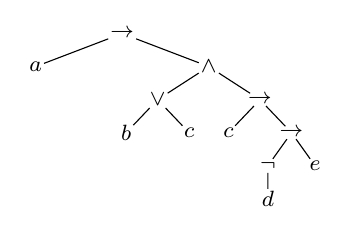
\begin{tikzpicture}[level distance=4.2mm,every node/.style={inner sep=0.6pt,font=\footnotesize},
level 1/.style={sibling distance=22mm},level 2/.style={sibling distance=13mm},level 3/.style={sibling distance=8mm},level 4/.style={sibling distance=6mm}]
\node{$\to$} child{node{$a$}} child{node{$\wedge$} child{node{$\vee$} child{node{$b$}} child{node{$c$}}} child{node{$\to$} child{node{$c$}} child{node{$\to$} child{node{$\neg$} child{node{$d$}}} child{node{$e$}}}}};
\end{tikzpicture}\par}
\sub{First-order logic}
\begin{itemize}
\item Predicates (formula level): $a$/2, $b$/3, $d$/1, $e$/1.
\item Functions (inside terms): $c$/2, $f$/2, $g$/1.
\item Free: $x,y$ (in $a(x,y)$, $e(f(x,g(y)))$) and $z$ (never bound).
\end{itemize}
\sub{Planning ($pX1_3$ = \texttt{posX-1-3}, $L2_3$ = \texttt{L-2-3})}
\begin{itemize}
\item Init: $pX1_0\wedge\neg pX2_0\wedge\neg pX3_0\wedge pY1_0\wedge\neg pY2_0\wedge\neg pY3_0$.
\item Goal: $pX2_5\wedge pY3_5$.
\item Frame axioms, posX at $t=3$:
\begin{itemize}
\item $(\neg pX1_3\wedge pX1_4)\to L2_3$;\ \ $(pX1_3\wedge\neg pX1_4)\to R1_3$
\item $(\neg pX2_3\wedge pX2_4)\to R1_3\vee L3_3$
\item $(pX2_3\wedge\neg pX2_4)\to R2_3\vee L2_3$
\item $(\neg pX3_3\wedge pX3_4)\to R2_3$;\ \ $(pX3_3\wedge\neg pX3_4)\to L3_3$
\end{itemize}
\item Up, $t=2$:
\begin{itemize}
\item $U1_2\to pY1_2\wedge\neg pY1_3\wedge pY2_3$
\item $U2_2\to pY2_2\wedge\neg pY2_3\wedge pY3_3$
\item $\neg U3_2$ (precondition $Y<3$ false)
\end{itemize}
\end{itemize}
\sub{Fuzzy}
\begin{itemize}
\item Average: not a T-norm: $T(0,1)=0.5\neq0$.
\item $(a\to b)\vee c$: $a\le b\Rightarrow1$; $\max(1,0.1)=1$.
\item $a\wedge b\to c$, $c\to a$, $b=.3$, $c=.1$, $a=0$: $a=.1$, then all satisfied.
\item Weighted MAX SAT: NP-hard. With $[0,1]$ values: PSL, polynomial.
\item PSL $\{a\}[1],\{\neg a,\neg b\}[2],\{b\}[3]$: $a=0$, $b=1$, value 5.
\end{itemize}
\sub{FCA (ME, W, M, I, R, Fe, E)}
\begin{itemize}
\item Aragorn = Boromir: clarify. ME is a full column.
\end{itemize}
\begin{itemize}
\item Object intents: Fr\{ME,R,Fe\}, Ar=Bo\{ME,W,Fe\}, Ga\{ME,W,M,I,Fe\}, Le\{ME,W,I,Fe\}, Sa\{ME,M,I,R,E\}, Go\{ME,R,E\}.
\item Their pairwise intersections add \{ME\}, \{ME,Fe\}, \{ME,R\}, \{ME,I\}, \{ME,M,I\}.
\end{itemize}
\textbf{Table of concepts} (every intent also contains ME)\\[1pt]
\begin{tabular}{@{}r|l|l|l@{}}
\# & intent & extent & below\\\hline
1 & ME & all 7 & (top)\\
2 & Fe & Fr Ar Ga Le Bo & 1\\
3 & R & Fr Sa Go & 1\\
4 & I & Ga Le Sa & 1\\
5 & W Fe & Ar Ga Le Bo & 2\\
6 & R Fe & Fr & 2, 3\\
7 & R E & Sa Go & 3\\
8 & M I & Ga Sa & 4\\
9 & W I Fe & Ga Le & 4, 5\\
10 & W M I Fe & Ga & 8, 9\\
11 & M I R E & Sa & 7, 8\\
12 & all 7 attributes & $\emptyset$ & 6, 10, 11\\
\end{tabular}\par
{\centering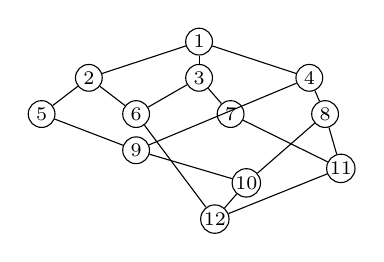
\begin{tikzpicture}[x=10mm,y=4.6mm,every node/.style={font=\scriptsize,inner sep=0.4pt}]
\foreach \n/\x/\y in {1/2/5,2/0.6/4,3/2/4,4/3.4/4,5/0/3,6/1.2/3,7/2.4/3,8/3.6/3,9/1.2/2,10/2.6/1.1,11/3.8/1.5,12/2.2/0.1}
  \node[circle,draw,minimum size=3.4mm] (c\n) at (\x,\y) {\n};
\foreach \a/\b in {1/2,1/3,1/4,2/5,2/6,3/6,3/7,4/8,4/9,5/9,9/10,8/10,8/11,7/11,6/12,10/12,11/12}
  \draw (c\a)--(c\b);
\end{tikzpicture}\par}
\begin{itemize}
\item Fe $\to$ c2; Magic $\to$ c8; Warrior $\to$ c5.
\item $(\{Ga,Sa\},\{M,I\})$: no, $\{Ga,Sa\}\up=\{ME,M,I\}$.
\item $(\{Fr,Ar\},\{Fe\})$: no, $\{Fe\}\dn$ has 5 objects.
\item $\{W,Fe\}\to\{I\}$: invalid (Aragorn, Boromir); $s=2/7$, $c=1/2$.
\item $\{R,Fe\}\to\{\neg E\}$: holds (Frodo); $s=1/7$, $c=1$.
\end{itemize}

%=====================================================================
\sect{15 Proof templates}
\begin{itemize}
\item \kw{Galois}: $Y\subseteq A\up\iff A\subseteq Y\dn$.
\item \kw{Antitone}: $m$ shared by all of $X'\supseteq X$ is shared by $X$.
\item \kw{$\alpha\beta\alpha=\alpha$}: $\supseteq$ extensive; $\subseteq$ antitone on $X\subseteq X\up{}\dn$.
\item \kw{Meet is a concept}: $(Y_1\cup Y_2)\dn=Y_1\dn\cap Y_2\dn=X_1\cap X_2$.
\item \kw{Anti-monotone}: $Y_1\subseteq Y_2\Rightarrow\sigma(Y_1)\ge\sigma(Y_2)$.
\item \kw{min largest}: $T(a,b)\le T(a,1)=a$, same for $b$.
\item \kw{English$\to$FOL}: ``all $A$ are $B$'' $\forall x(A\impl B)$; ``some'' $\exists x(A\wedge B)$.
\item Friends of John know one of his children:\\$(\forall x)(fr(x,j)\impl(\exists y)(ch(y,j)\wedge kn(x,y)))$.
\end{itemize}

\sect{16 Worked slide examples}
\ex{\textbf{Prop.\ resolution} $((A\impl B)\wedge(B\impl C))\impl\neg(\neg C\wedge A)$
\begin{itemize}
\item Goal line: $\gd{\neg(\ldots)}$ gives $\gd{(A\impl B)\wedge(B\impl C)}$, $\gd{\neg C\wedge A}$.
\item Lines: $\gd{\neg A,B}$, $\gd{\neg B,C}$, $\gd{\neg C}$, $\gd{A}$.
\item Resolve: $\gd{B}$, then $\gd{C}$, then $\gd{}$. Valid.
\end{itemize}}
\ex{\textbf{FOL resolution} $(\exists x)(A\wedge\neg P(x))\impl\neg(\forall x)P(x)$
\begin{itemize}
\item Negate: $(\exists x)(A\wedge\neg P(x))$ and $(\forall x)P(x)$.
\item Skolemize: $A$, $\neg P(c)$; drop $\forall$: $P(x)$.
\item Unify $x=c$: $\gd{}$. Valid.
\end{itemize}}
\ex{\textbf{Prenex} $(\exists x)(\forall y)R(x,y)\impl(\forall y)(\exists x)R(x,y)$
\begin{itemize}
\item Rename: $\ldots\impl(\forall u)(\exists v)R(v,u)$.
\item $(\forall x)(\exists y)(\forall u)(\exists v)(R(x,y)\impl R(v,u))$ (antecedent flips).
\item Skolemize: $y=f(x)$, $v=g(x,u)$.
\end{itemize}}
\ex{\textbf{Fuzzy} (slides): product $R(.9,.2)=.2/.9\approx.22$; $I(.22\wedge.9)=.198$. Mamdani: HOT .9, CROWDED .6 $\Rightarrow\alpha=.6$.}
\ex{\textbf{MAX SAT} $\{s\}[7]$, $\{\neg s,\neg b\}[8]$, $\{b\}[10]$
\begin{itemize}
\item Worlds $(s,b)$: $(0,1)=18$, $(1,0)=15$, $(1,1)=17$, $(0,0)=8$.
\end{itemize}}
\ex{\textbf{Forward chaining} B, C true; prove H
\begin{itemize}
\item R1 BDE$\to$F, R2 DG$\to$A, R3 CF$\to$A, R4 C$\to$D, R5 D$\to$E, R6 A$\to$H, R7 B$\to$X, R8 XC$\to$A.
\item First rule: D, E, F, A, H. Last rule: X, A, H.
\end{itemize}}

\sect{17 Exam recipes (step by step)}
\begin{itemize}
\item \kw{When is $F$ false?} Main connective first: $X\to Y$ false iff $X=1,Y=0$; split cases; list all rows.
\item \kw{CNF} \cnt{3}: \n1remove $\impl$ \n2push $\neg$ inward \n3distribute $\vee$ over $\wedge$; drop clauses with $p,\neg p$.
\item \kw{Unsat KB, 2 ways}: truth table; resolution to $\gd{}$.
\item \kw{Frame axioms}: for each grounded fluent, 2 axioms (becomes true, becomes false); RHS = actions with that effect.
\item \kw{Action constraint}: one per grounding; impossible precondition $\Rightarrow\neg a_t$.
\item \kw{Concept check} \cnt{2}: $A\up=B$? $B\dn=A$? Closure of $m$: $\{m\}\dn{}\up$.
\item \kw{Implication} $Z_1\to Z_2$: does every object of $Z_1\dn$ have $Z_2$? Then $s$, $c$.
\item \kw{T-norm?} Test the 4 axioms; first try $T(a,1)=a$.
\item \kw{R-implication}: $x\le y\Rightarrow1$; else T-norm's formula.
\item \kw{Fuzzy inference}: raise each conclusion to $\phi$(premises); repeat until stable.
\item \kw{PSL}: write each clause term; case split where $\min(\cdot,1)$ changes; maximize.
\item \kw{DL instance}: unfold the definition; witness for each $\exists$; requires $\equiv$.
\item \kw{DL subsumption}: take $x\in C^I$, show $x\in D^I$; or $C\sqcap\neg D$ unsat.
\item \kw{$\lambda$ reduction}: leftmost outer redex first; rename before substituting.
\end{itemize}
\end{multicols*}
\end{document}
